\documentclass[11pt]{article}
\usepackage[utf8]{inputenc}
\usepackage[russian]{babel}
\usepackage[T1]{fontenc}
\usepackage{amssymb,amsmath,clrscode,graphicx,indentfirst}

\author{Олег Смирнов}
\title{Курс kiev-clrs -- Лекция 12. Списки с пропусками}
\date{20 июня 2009 г.}

\begin{document}
\maketitle
\tableofcontents

\newpage
\setlength{\parskip}{1ex plus 0.5ex minus 0.2ex}
\section{Цель лекции}
\begin{itemize}
\item Рассмотреть списки с пропусками
\item Рассмотреть анализ ``с высокой вероятностью''
\end{itemize}

\section{Связные списки и списки с пропусками}
Список с пропусками является структурой данных, аналогичной сбалансированным деревьям:
\begin{itemize}
\item RB-деревья
\item декартовы деревья (treaps)
\item B-деревья
\end{itemize}
Операций поиска, вставки и удаления работают в списке с пропусками за время $\lg(n)$ для $n$ элементов \emph{с большой вероятностью}.

Списки с пропусками были предложены в 1990 году~\cite{Pugh90skiplists}. Отличительной особенностью этой структуры является простота имплементации.

Сортированный связный список является простейшей структурой со временем поиска $\Theta(n)$. Работу такой структуры можно улучшать разными способами. Одной из идей является добавление еще одного уровня (связного списка), обеспечивающего быстрый доступ через несколько элементов.
\begin{figure}[ht]
  \centering
  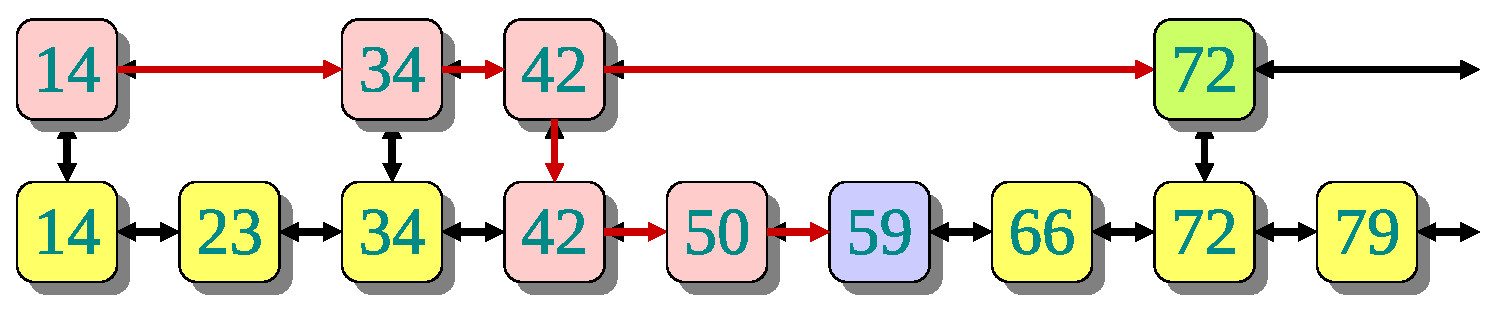
\includegraphics[width=4in]{lecture12/linklists.eps}
  \caption{Связные списки}
  \label{fig:linklists}
\end{figure}
Хорошим примером такой структуры является метро с экспресс-линией между несколькими удалеными станциями и местной линией, которая останавливается на каждой станции.

Итак, на нижнем уровне $L_2$ присутствуют все элементы, на верхнем $L_1$ -- только некоторое количество. Между одинаковыми элементами уровней существуют ссылки. Это инвариант структуры.

В таком случае алгоритм поиска $Search(x)$ будет состоять из шагов:
\begin{enumerate}
\item Начало поиска в левом верхнем углу (на экспресс-линии)
\item Передвигаться вправо по верхнему списку $L_1$ пока это возможно ($x < $ ключа)
\item Переместиться в нижний список и передвигаться до искомого элемента $x$
\end{enumerate}

\subsection{Анализ поиска}
Скорость работы поиска будет зависить от количества элементов в верхнем списке $|L_1|$. Для анализа преположим, что в $L_1$ попало несколько элементов в случайном порядке. 

Тогда время поиска в худшем случае равно:
\begin{align*}
  \approx \underbrace{|L_1|}_{\text{в }L_1} + \underbrace{\frac{|L_2|}{|L_1|}}_{\text{в }L_2} =\\
  = |L_1| + \frac{n}{|L_1|} \\
  \text{(минимизируя)} \\
  |L_1|^2 = |L_2| = n \Rightarrow |L_1| = \sqrt{n}
\end{align*}
Итак:
\begin{equation*}
  |L_1| + \frac{|L_2|}{|L_1|} = \sqrt{n} + \frac{n}{\sqrt{n}} = 2\sqrt{n}
\end{equation*}
Полученная структура выглядит сбалансированной: на каждом уровне будут просмотрены цепочки одинаковой длины.
\begin{figure}[h!]
  \centering
  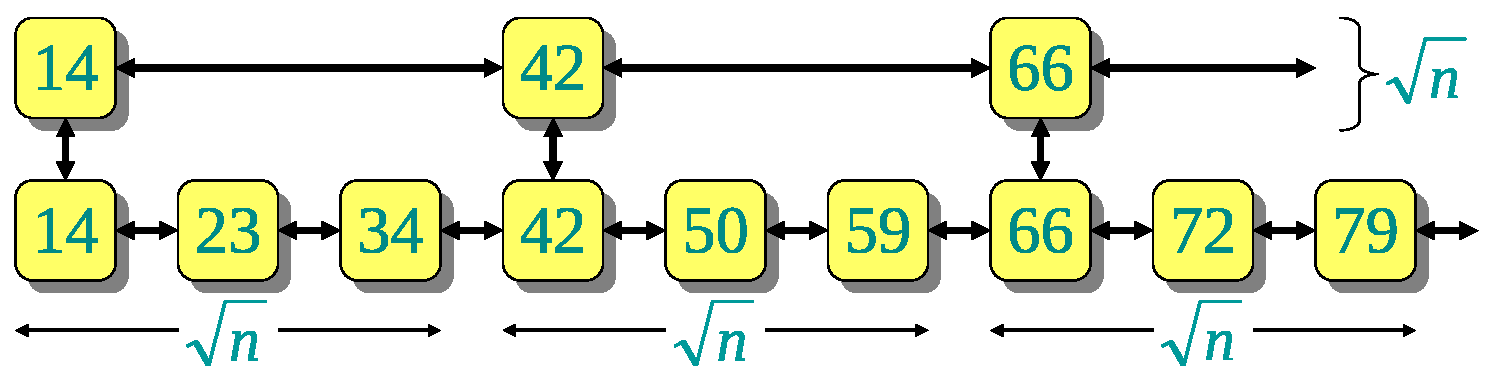
\includegraphics[width=4in]{lecture12/2linklists.eps}
  \caption{Связные списки}
  \label{fig:2linklists}
\end{figure}

Можно показать, что время поиска можно улучшать, добавляя новые экспресс-уровни:
\begin{itemize}
\item $2$ отсортированных списка $\Rightarrow 2\sqrt{n}$
\item $3$ отсортированных списка $\Rightarrow 3\sqrt[3]{n}$
\item $k$ отсортированных списка $\Rightarrow k\sqrt[k]{n}$
\item $\lg n$ отсортированных списка $\Rightarrow {\lg n}\sqrt[\lg n]{n} = {\lg n}\cdot{n^{\frac{1}{\lg n}}} = 2\lg n$
\end{itemize}

$\lg n$ сортированных связных списков ведут себя похоже на бинарное дерево. В идеальном списке с пропусками отношение количества элементов между уровнями постоянно и равно $2$. В этом случае в нижнем списке будет $2^{\lg n} = n$ элементов.
\begin{figure}[ht]
  \centering
  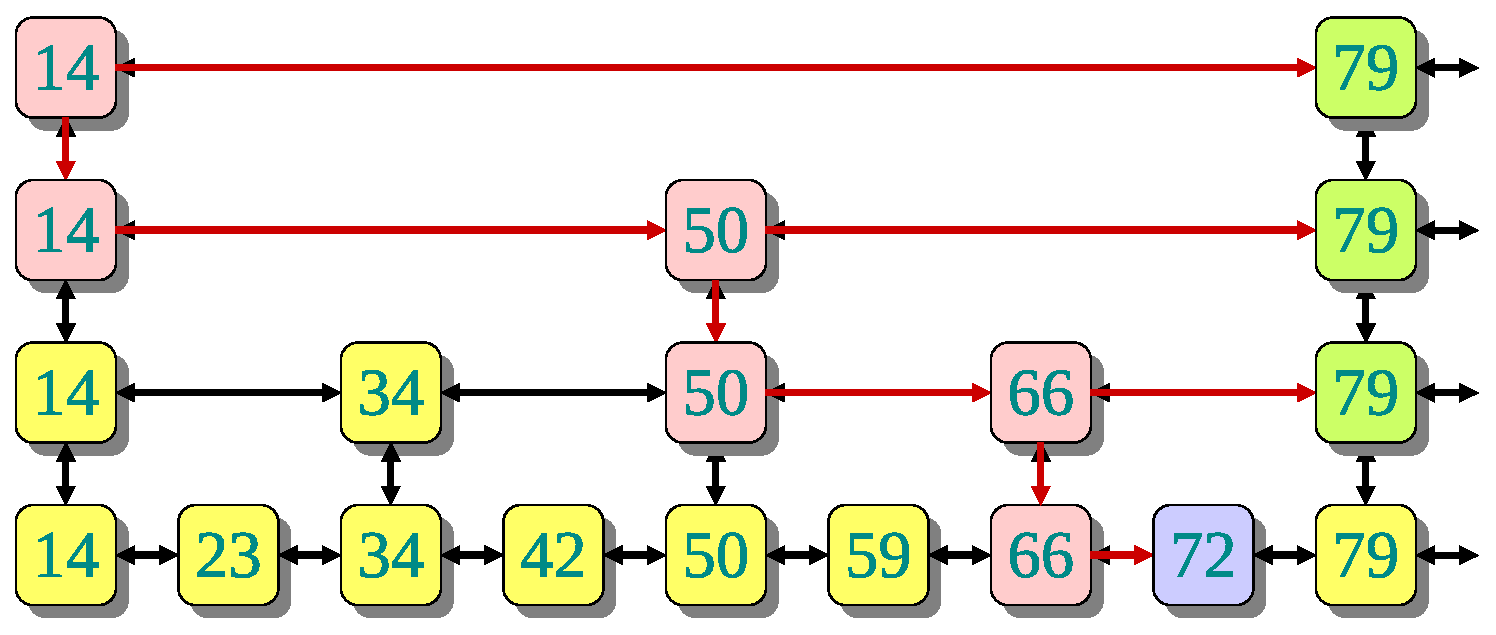
\includegraphics[width=4in]{lecture12/skiplist.eps}
  \caption{Идеальный список с пропусками}
  \label{fig:skiplist}
\end{figure}
Поиск в этой структуре будет выполнятся за $O(\lg n)$ шагов.

\section{Алгоритм поиска}
В практической реализации обычно добавляют специальные элементы-ограничители в начале каждого уровня. Их значение принимают равным $-\infty$.
\begin{figure}[ht]
  \centering
  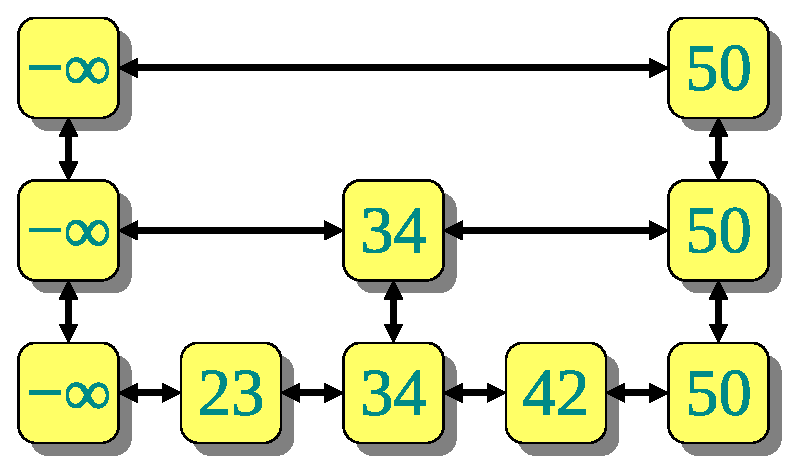
\includegraphics[width=2.2in]{lecture12/skiplist_inf.eps}
  \caption{Список с ограничителями}
  \label{fig:skiplist_inf}
\end{figure}

Алгоритм на псевдокоде:
\begin{codebox}
\Procname{$\proc{Search}(L, x)$}
\li $v \gets L$
\li \While $v \neq NULL$ and $key(v) \neq x$ 
\li \Do
\li \If $key(right(v)) > x$
\li   \Then $v \gets down(v)$
\li   \Else $v \gets right(v)$ 
    \End
  \End
\li \Return v
\end{codebox}

\section{Алгоритмы модификации}
Необходимо разработать алгоритмы вставки и удаления элемента, которые бы сохраняли свойства списка с пропусками и работали за логарифмическое время. Алгоритм вставки $Insert(x)$ включает следующие шаги:
\begin{itemize}
\item найти место для вставки в самом нижнем списке $Search(x)$
\item вставить элемент в нижний список (поддержка инварианта структуры)
\item ``бросить монетку'' и в зависимости от результата (например, если выпала ``решка'') добавить элемент уровнем выше (вероятность $1/2$)
\item повторять предыдущий шаг, уменьшая вероятность с каждым уровнем (бросая монетку при каждой вставке)
\end{itemize}
Таким образом, на нижний уровень элемент будет вставлен всегда, на уровень выше -- с вероятностью $1/2$, выше -- $1/4$ и т.д. Элемент попадет на уровень $\lg n$ с вероятностью $1/n$.

Алгоритм удаления элемента $Delete(x)$ тривиален: элемент удаляется из всех списков, которые его содержат.

\section{Анализ ``с высокой вероятностью''}
\textbf{Теорема:} каждый поиск в списке с пропусками из $n$ элементов \emph{с высокой вероятностью} выполняется за $O(\lg n)$.

Событие $E$ случается \emph{с высокой вероятностью}, если существует $\alpha \geqslant 1$, такое, что для выбранных соответствующим образом констант событие $E$ случается с вероятностью $\geqslant 1 - O(\frac{1}{n^{\alpha}})$. Константы в определениях связаны, т.е. если необходимо, чтоб условие поиска выполнялось с вероятностью  $1 - O(\frac{1}{n^{100}})$, то сам поиск будет выполнятся за время, предположим $O(100 \lg n)$, которое всё равно является логарифмическим.

В доказательстве используется неравеноство Буля:
\begin{equation*}
  Pr\{E_1 \cup E_2 \cup \ldots \cup E_k\} \leqslant Pr\{E_1\} + Pr\{E_2\} + \ldots + Pr\{E_k\}
\end{equation*}

\textbf{Лемма:} с высокой вероятностью кол-во уровней списка с пропусками равно $O(\lg n)$. 

Вероятность обратного события $Pr\{\# > c\lg n\}$ должна быть полиноминально малой:
\begin{align*}
  Pr\{\# > c \lg n \} \leqslant \\
  \text{(суммируем по всем элементам} \\
  \text{списка по неравенству Буля)} \\
  \leqslant n Pr\{X \text{ выше }c \lg n\} = \\
  = n {\left(\frac{1}{2}\right)}^{c\lg n} = \frac{n}{n^c} = \\
  = \frac{1}{n^{c-1}} = \frac{1}{n^\alpha} \\
  \text{выбирая }\alpha = c-1
\end{align*}
Информации о высоте уровней недостаточно. Для доказательства теоремы необходимо еще знать длину цепочек между элементами, соединяющими уровни списка.

Идея доказательства: рассмотреть ``обратный'' поиск от искомого элемента в левый верхний угол списка

Этот процесс будет выполнять в точности такое же кол-во шагов, что и прямой поиск:
\begin{itemize}
\item поиск начинается с элемента в нижнем списке
\item каждое перемещение между элементами происходит влево или вверх по списку
\item переход влево происходит, когда у текущего элемента нет соседа сверху (при построении выпал ``орел'')
\item переход вверх происходит, когда сосед есть (выпала ``решка'')
\item поиск останавливается в корне или в $-\infty$
\end{itemize}
Для доказательства общего случая достаточно доказать, что каждый поиск выполнятся за логарифмическое время с высокой вероятностью. Тогда общий случай будет получен из неравенства Буля.
\begin{enumerate}
\item Поиск остановится, когда будет достигнут корень структуры
\item Количесво переходов вверх в поиске $<$ кол-ва уровней $\leqslant c \lg n$ с высокой вероятностью (по лемме)
\item Переход вверх выполнятся с вероятностью $1/2$ (по построению списка)
\item Следовательно, общее количество переходов $\leqslant$ вероятности построения уровня высотой $c \lg n$ (количеству подбрасываний монетки для получения $c \lg n$ ``решек'')
\end{enumerate}
Т.о. необходимо доказать, что количество подбрасываний монетки, необходимое для получения $c \lg n$ ``решек'' равно $\Theta(\lg n)$ с высокой вероятностью.

Можно доказать для частного случая границу $O(\lg n)$: рассмотрим $10 c \lg n$ подбрасываний монетки. Когда выпадет ровно $c \lg n$ решек?
\begin{align*}
  Pr\{\# c \lg n\text{ решек}\} = 
  \underbrace{\binom{10 c \lg n}{c \lg n}}_{\text{перестановки}} \cdot
  \underbrace{{\left(\frac{1}{2}\right)}^{c\lg n}}_{\text{решки}} \cdot
  \underbrace{{\left(\frac{1}{2}\right)}^{9c\lg n}}_{\text{орлы}} \\
  Pr\{\# c \lg n\text{ решек}\} \leqslant \binom{10 c \lg n}{c \lg n} \cdot
  {\left(\frac{1}{2}\right)}^{9c\lg n} \leqslant \\
  \leqslant {\left(e\frac{10 c \lg n}{c \lg n} \right)}^{c\lg n} \cdot
  {\left(\frac{1}{2}\right)}^{9c\lg n} = \\
  = {(10 e)}^{c \lg n} 2^{-9c\lg n} = \\
  = 2^{\lg{(10 e)}\cdot c \lg n}2^{-9c\lg n} = \\
  = 2^{(\lg{(10 e)}-9) \cdot c \lg n} = 1 / n^\alpha \\
  \text{для }\alpha = (9-\lg{(10 e)}) \cdot c
\end{align*}
Таким образом $Pr\{\text{не более }c \lg n\text{ решек}\} \leqslant 1/n^\alpha$, для $\alpha = (9-\lg{(10 e)}) \cdot c$. Здесь $\alpha \to \infty$ при $10 \to \infty$ для любого $c$.

Таким образом константа, скрытая внутри границы $O(\lg n)$ удовлетворяет требование для $\alpha$.

\section{Заключительные замечания}
\begin{itemize}
\item с теоретической точки зрения список с пропусками ничем не лучше сбалансированного бинарного дерева. С практической точки зрения эта структура намного проще в реализации
\item cписки с пропусками широко используются в пиринговых сетях для реализации распределенных хэш-таблиц \cite{Stoica01chord:a} \cite{1124030} \cite{Harvey03skipnet:a}
\end{itemize}

\bibliographystyle{alpha}
\bibliography{lecture12}

\end{document}
